\documentclass[a4paper, 12pt]{article}
\usepackage{comment} 
\usepackage{fullpage}
\usepackage[hidelinks]{hyperref}
\usepackage{amsmath}
\usepackage{environ}
\usepackage{graphicx}
\usepackage{tabto,enumitem}


\begin{document}
\noindent
\large\textbf{SOEN 6011} \hfill \textbf{Aniket Tailor}\\
\large\textbf{Software Engineering Processes} \hfill \textbf{40195068} \\
Function 8 : Standard Deviation $\sigma$ \hfill Date: 5 August 2022\\
\normalsize Problem 4 \\


\section{Error \& Exception Handling}

\begin{itemize}
    \item Error management makes it possible to gracefully handle both hardware and software problems and enables interrupted execution to continue. Either the programmer creates the necessary codes to handle problems or uses software tools to handle errors when it comes to error handling in software. When mistakes cannot be categorised, they are typically handled by returning unique error codes. For some applications, there exist specialised programs called error handlers that can assist in handling errors. These programs can foresee errors, assisting in recovery without actually terminating the program. 
    \item Responding to undesirable or unexpected events that occur while a computer program is running is known as exception handling. Without this process, exceptions would interfere with a program's regular functioning and cause it to crash. Exception handling deals with these events to prevent this from happening.
    \item In the given source code to find standard deviation, all the error and exception handling have been taken care of. To summarize a few exception handling errors, 
    \begin{enumerate}
        \item User cannot enter string as input. 
        \item If while entering the numerical data values, user enters a string by error then he/she will be prompted to enter the number again at that index value.
        \item User will need to re-enter the size of the array if it is 0.
        \item User should enter at-least two numbers, in order to find Standard Deviation.
        \item If all the elements of the array are same then it should given output as 0.
    \end{enumerate}
\end{itemize}

\newpage
\section{Debugger}
Debugging let you run a program interactively while keeping an eye on the variables and source code as they are being used. A break point in the source code indicates when the program's execution should halt while being fixed. Once the program has been paused, variables can be examined, their contents can be changed, etc. You can launch a Java program in Debug mode using Eclipse. Eclipse has a Debug viewpoint that offers you a ready-made selection of views. And through debug commands, Eclipse enables you to manage the execution flow.
\subsection{Advantages of debugger}
\begin{itemize}
    \item Debugging helps in solving the unknown problems in the code For example, compile time and run time exceptions.
    \item We can step into and out of the Eclipse debugger and check the dependencies of other variables with regard to the currently skipped variable.
    \item Debugging is a very useful tools for inspecting the state of the objects and variables in your code at run time.
\end{itemize}
\subsection{Disadvantages of debugger}
\begin{itemize}
    \item While in certain IDE's debuggers we can backtrack the debugger and examine its prior value, the Eclipse debugger does not allow us to do this.
    \item When multiple threads are active at once, debuggers frequently become stuck and refuse to advance.\\
    
\begin{figure}[h]
    \centering
    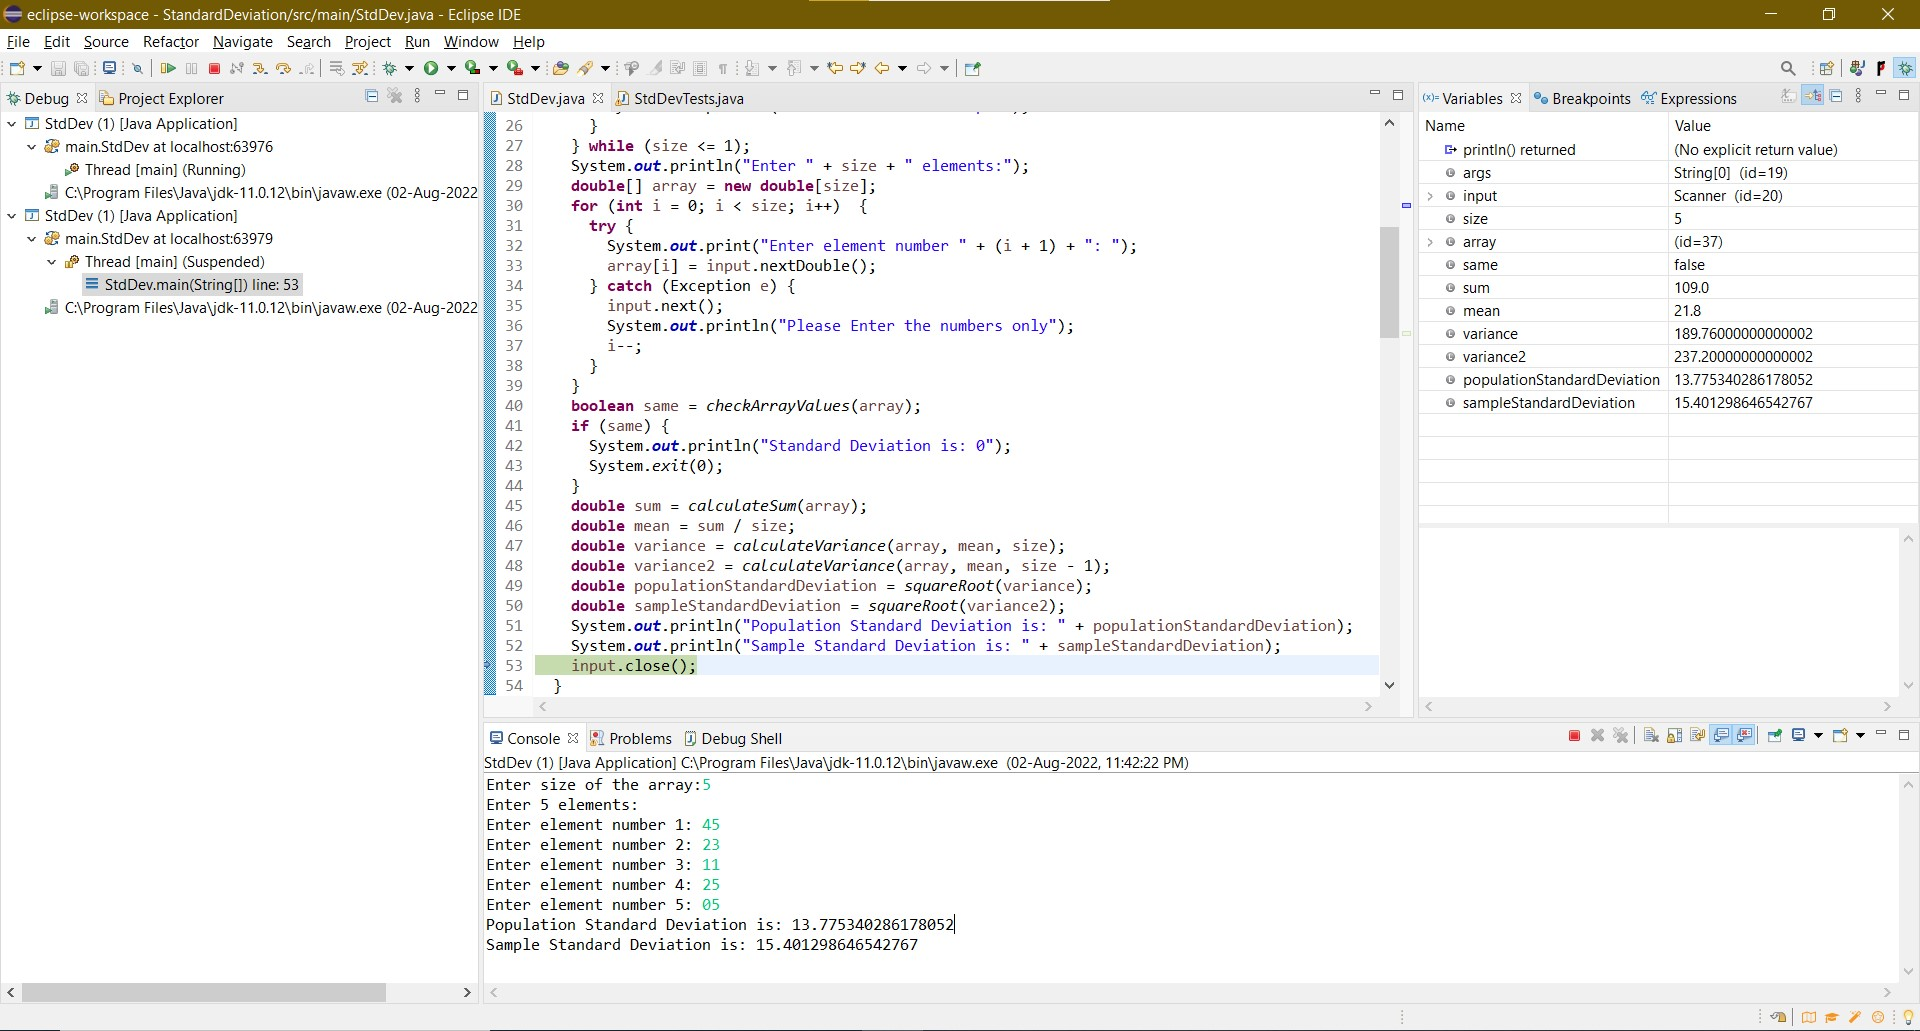
\includegraphics[width=0.90\linewidth]{Images/Debugger.jpg}
    \caption{Debugger in use}
    \label{fig:Debugger Image}
\end{figure}
\end{itemize}

\newpage
\section{Checkstyle}
Programmers can use Checkstyle as a development tool to write Java code that follows a coding standard. To relieve humans of this tedious work, it automates the process of checking Java code. It is therefore perfect for initiatives that aim to impose a coding standard. It may examine a variety of elements in your source code. It can identify issues with class and method design. It can also check for formatting and code layout problems.
\subsection{Advantages of Checkstyle}
\begin{itemize}
    \item Portable between IDEs [Eclipse And IntelliJ]
    \item Due to the fact that check style was truly intended to be an independent framework, integrating it with your external tools is considerably simpler.
    \item It lets you format the code with respect to global standards. 
    \item Ability of creating your own rules. Eclipse defines a large set of styles, but checkstyle has more, and you can add your own custom rules.

\end{itemize}
\subsection{Disadvantages of Checkstyle}
\begin{itemize}
    \item Removes the ability to do any 'special-case' formatting where an alternate format would make code more readable.
    \item The checks done by checkstyle do not confirm the correctness or completeness of the code.
    \item It ties you into using IDEs which support exactly the reformatting features you need.
    
\begin{figure}[h]
    \centering
    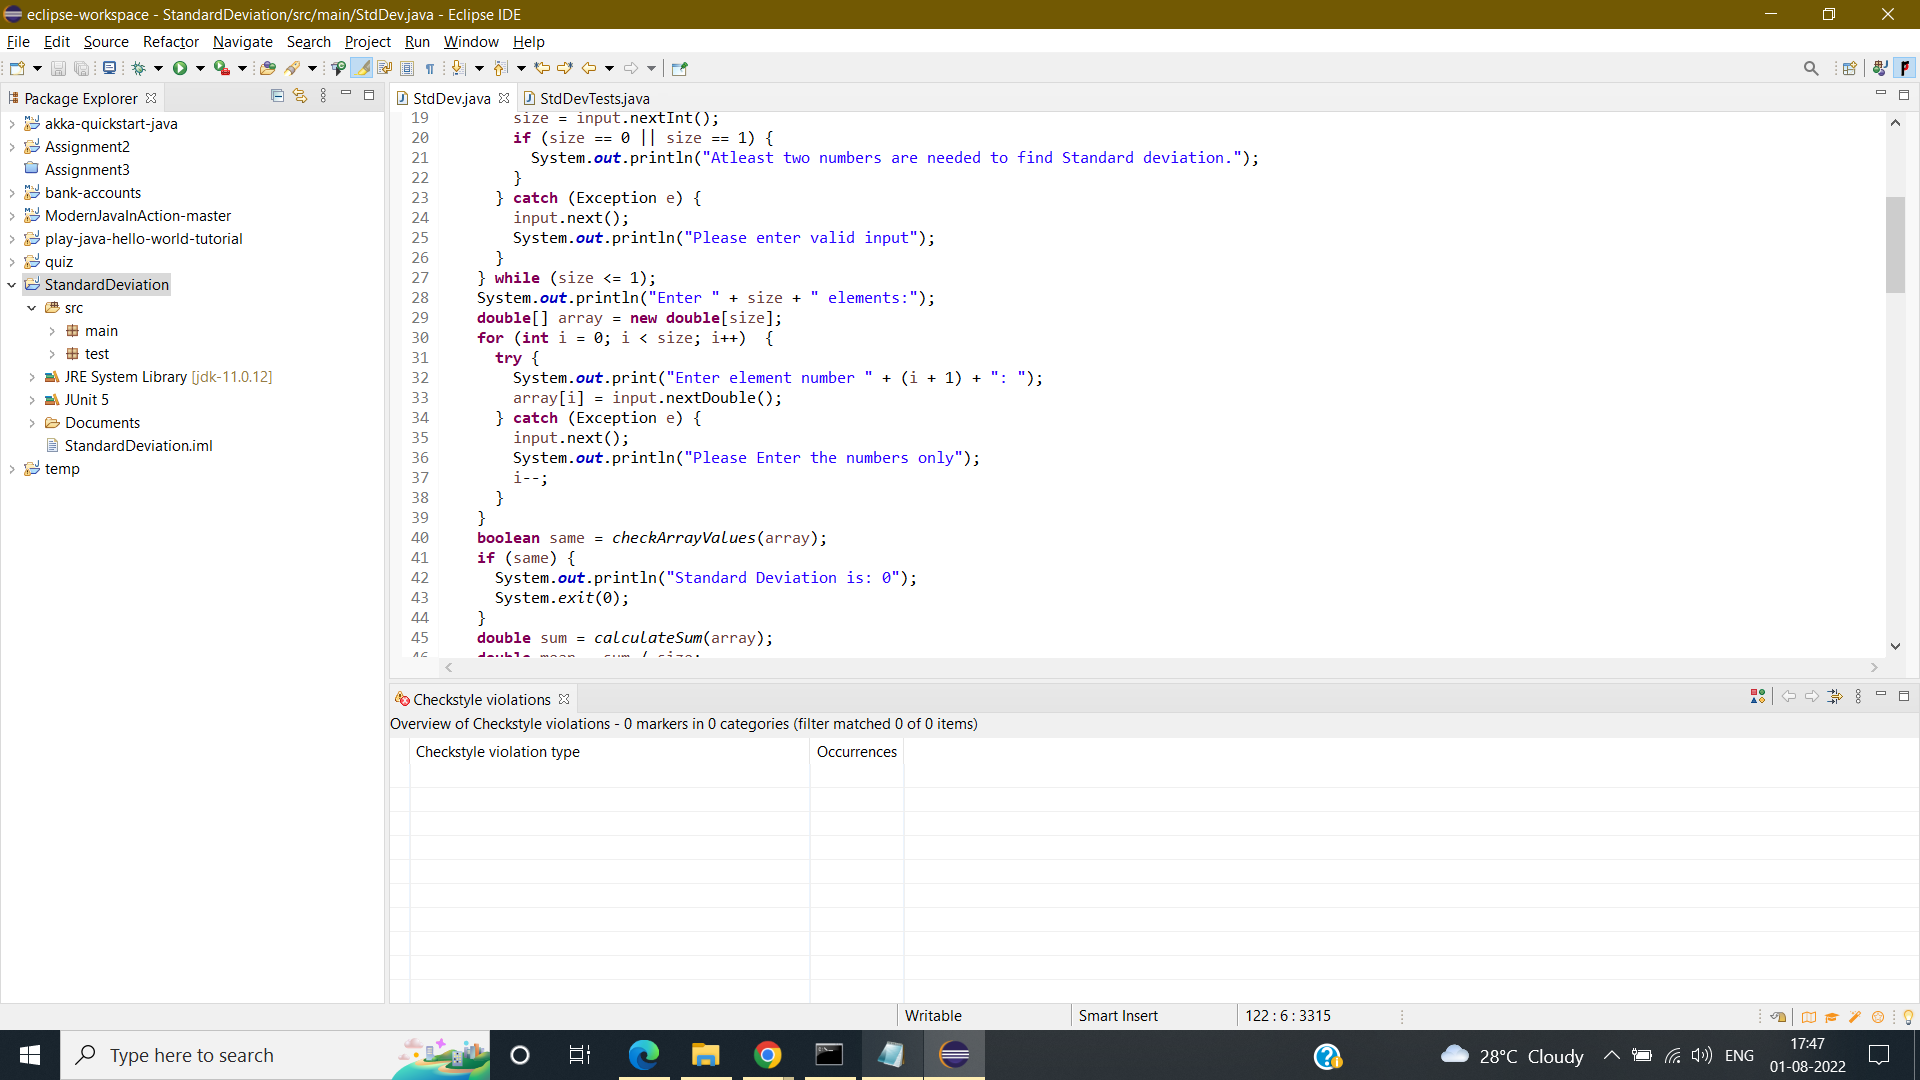
\includegraphics[width=0.87\linewidth]{Images/Checkstyle.png}
    \caption{Checkstyle in use}
    \label{fig:Checkstyle Image}
\end{figure}
\end{itemize}

\newpage
\begin{thebibliography}{15}

\addcontentsline{toc}{chapter}{Bibliography}
\bibitem{1}
\href{https://www.techtarget.com/searchsoftwarequality/definition/error-handling}{https://www.techtarget.com/searchsoftwarequality/definition/error-handling}

\bibitem{2}
\href{https://www.techopedia.com/definition/16626/error-handling}{https://www.techopedia.com/definition/16626/error-handling}

\bibitem{3}
\href{https://checkstyle.sourceforge.io/}{https://checkstyle.sourceforge.io/}

\bibitem{4}
\href{https://softwareengineering.stackexchange.com/questions/92256/advantages-and-disadvantages-of-forced-code-reformat}{https://softwareengineering.stackexchange.com/questions/92256/advantages-and-disadvantages-of-forced-code-reformat}

\end{thebibliography}
\end{document}
